\section{合成方法与实验条件比较}
\label{sec:condition-matrix}

本节先概括前人实验得到的规律，再按主要相形成过程比较各合成方法。表格逐项列出原料与配比、热历史、气氛与体系、容器与助熔剂、冷却或生长程序以及产物表征。比较的目的不在于组合出推荐配方，而在于保留不同研究对象之间的差异。目标相的直接文献仅明确了开放体系高温溶液法和单晶X射线结构鉴定；投料、温度程序、坩埚、助熔剂和冷却程序均无明确记载，因此记为未报道\cite{ababaikeri2024ba5y12zn}。

\subsection{前人实验的主要结论}

已有实验表明：第一，组成坐标比单一的最高温度更能解释Ba--Y--Si--O体系的相形成差异，Y$_2$O$_3$\slash SiO$_2$比、MoO$_3$用量和冷却速率共同影响结构类型和晶体质量\cite{kolitsch2009crystal,wierzbickawieczorek2017high}；第二，单晶结构不能代表块体相纯，无Zn陶瓷研究仍检测到第二相\cite{yamane2024microstructure,gulay2024navigation}；第三，局部相图可将复现问题转化为可检验的相区问题，并为下一轮投料提供依据\cite{gulay2024navigation}。下文据此比较各路线的实验条件，不将这些相关体系的结果直接改写为目标相的配方。

\subsection{合成条件的统一比较}

图~\ref{fig:route-matrix}\CJKecglue{}将文献记录分为“合成方法--实验条件--产物表征”三个层次。外加助熔与自熔/熔体路线列出助熔剂比例、容器接触、冷却与分离、熔体均化和成核条件；固相陶瓷路线列出混合、压片、煅烧、复磨和复烧条件；仅在文献明确报道机械活化时才列入机械化学路线；Czochralski路线另列籽晶、提拉、旋转和退火条件。图中连线表示实验条件与表征结果的对应关系，不表示某一变量必然导致特定相。

\begin{figure*}[t]
  \centering
  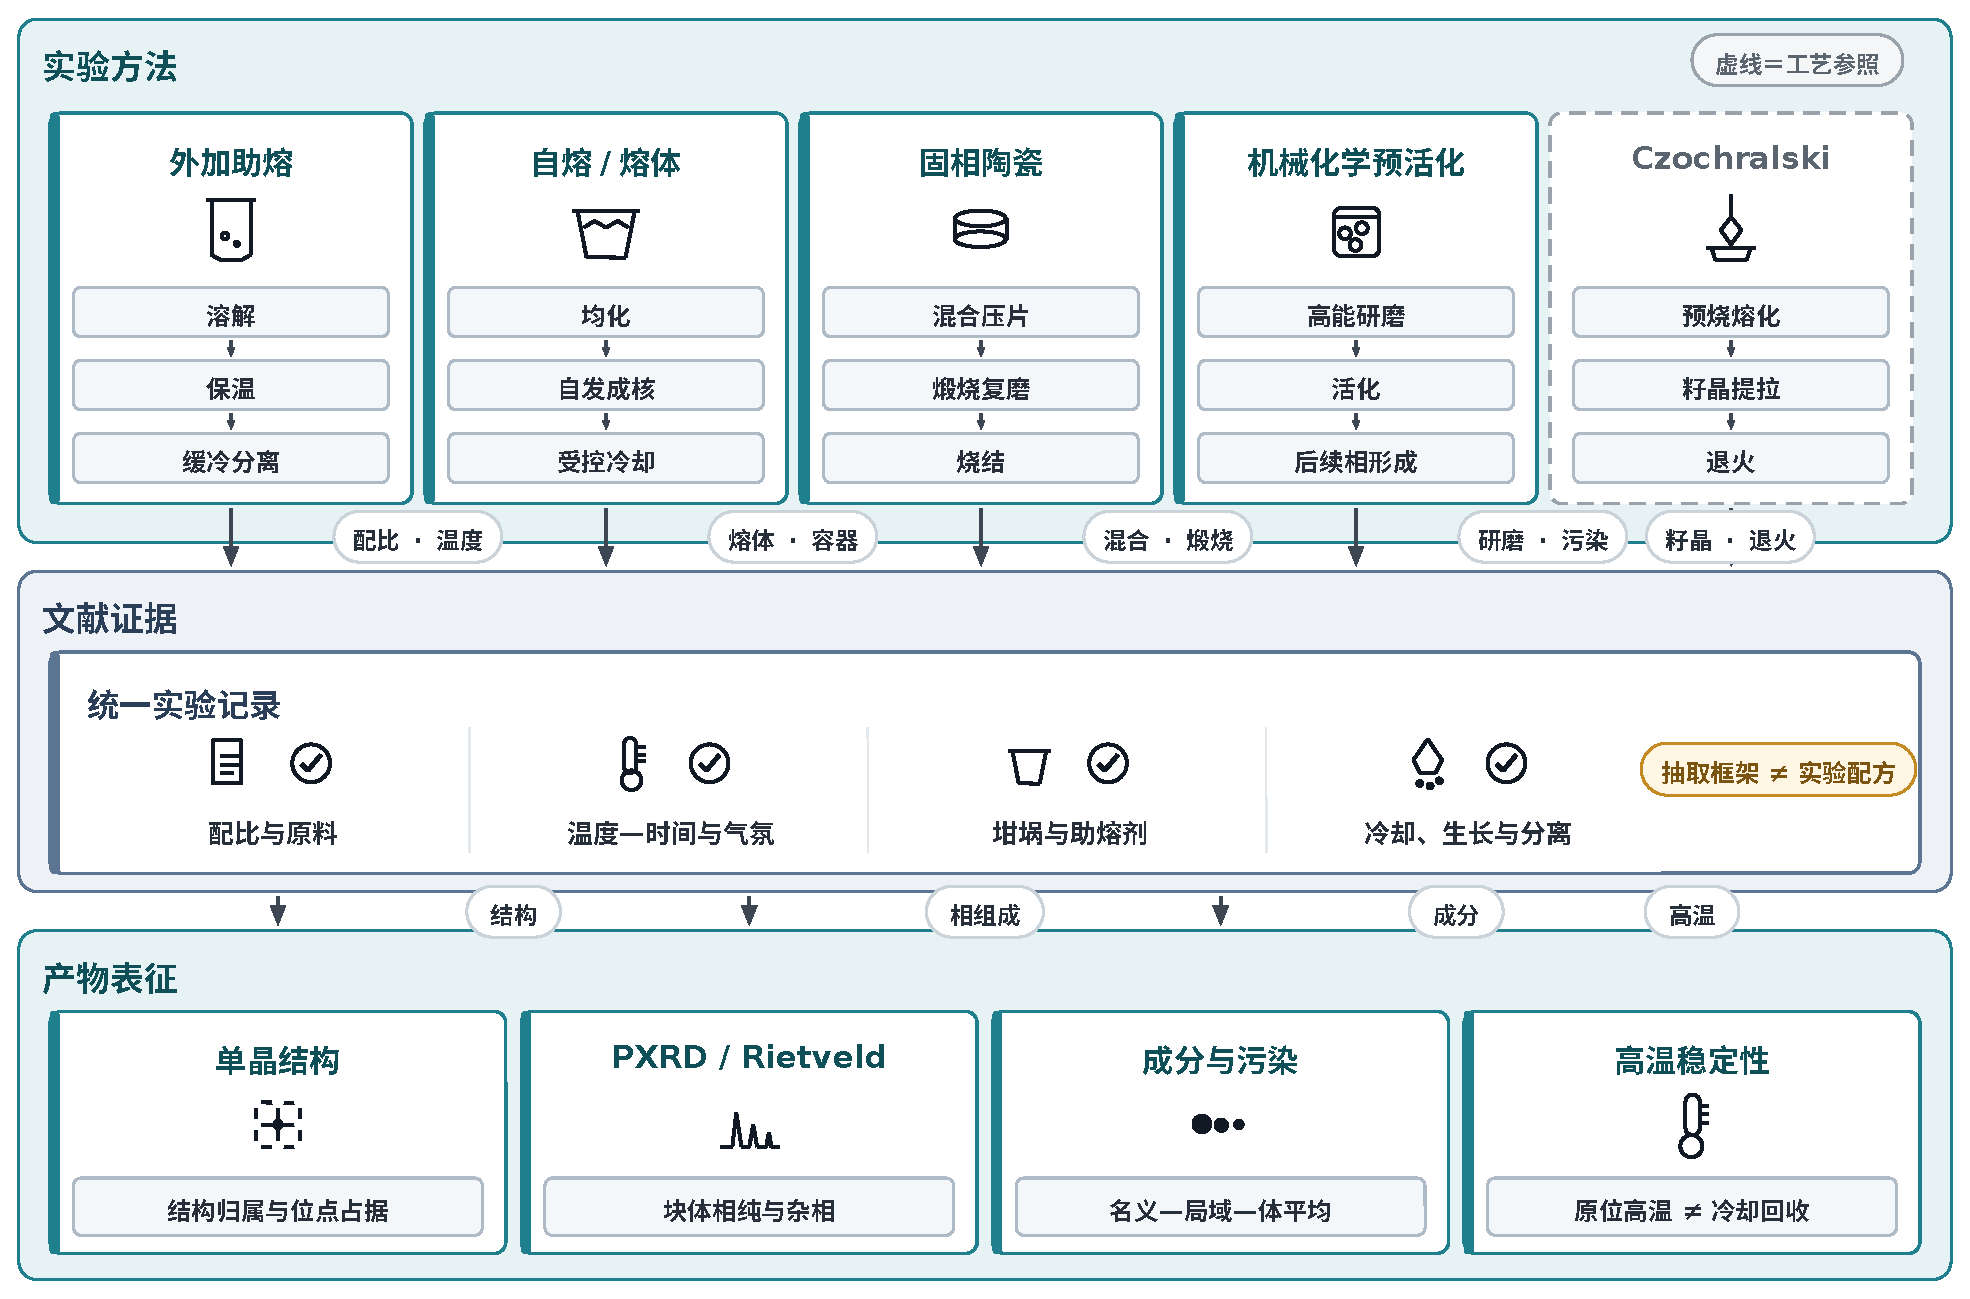
\includegraphics[width=\textwidth]{../figures/pdf/fig02_route_variable_matrix.pdf}
  \caption{\textbf{不同合成方法的条件比较与产物表征。}左侧区分外加助熔、自熔/熔体、固相陶瓷、机械化学预活化和Czochralski路线；中部列出可比较的原料、热历史、气氛、容器、冷却和生长条件；右侧列出单晶结构、PXRD\slash Rietveld精修、成分分析及高温稳定性等互补表征。连线表示实验条件与表征结果的对应关系，不表示变量与相形成之间的因果关系；Czochralski路线仅作工艺参照，本图不构成目标相的实验配方。}
  \label{fig:route-matrix}
\end{figure*}

各方法的文献数量并不代表其条件记录同样完整。只有在来源明确说明时，才能确认无坩埚熔体法、开放体系高温溶液法或稀土硅酸盐高温结晶等路线\cite{christensen1994investigation,ababaikeri2024ba3zn4si4o15,leonyuk1999high,giess1982zn2sio4}。Leonyuk的另一条题名级记录仅确认单晶对象和结构精修，不能据此判断生长方法\cite{leonyuk1999crystal}。固相反应文献涵盖结构相变、陶瓷烧结、掺杂表征和玻璃析晶，但仅有可定位到实验段落的项目才列入数值表格\cite{lin1999phase,zou2021crystal,kerstan2012thermal,cai2024optimized,zhao2026crystal,tejas2024structural,pires2001luminescence,kerstan2015kristallphasen}。机械化学资料中，Tzvetkov与Minkova明确报道了机械处理；Yıldırım仅报道助剂参与的固--液相烧结，不能因研究对象为粉体而归为机械化学\cite{tzvetkov2001effects,yldrm2009y2sio5}。提拉法资料同样仅作为Y$_2$SiO$_5$\slash Ln$_2$SiO$_5$的工艺参照\cite{pang2005study,alizadeh2021spectroscopy,shoudu1999czochralski,brandle1986czochralski}。

\subsection{条件总表}

表~\ref{tab:synthesis-conditions}\CJKecglue{}逐行列出每条记录的文献出处、化学输入、合成方法、与目标相的关系，以及热历史、体系、坩埚与助熔剂、冷却或生长程序、产物表征和未记载项。表~\ref{tab:synthesis-conditions-b}\CJKecglue{}以相同编号承接热历史、气氛与体系、坩埚与助熔剂、冷却或生长程序、产物表征和未记载项。来源与出处栏标注“实验部分”时，表示本文已核对原始实验段落；标注“摘要/题名”时，仅确认其中明示的对象或方法，不由“晶体生长”等泛称补出未写明的步骤。“—”表示本次核查未取得该项目的明确记载，不表示原实验没有该步骤。

% >>> condition-matrix (generated by tools/zh_table_merge.py)
\Needspace{8\baselineskip}
{\fontsize{8}{9.8}\selectfont\setlength{\tabcolsep}{3pt}\renewcommand{\arraystretch}{1.05}
\begin{longtable}{P{\dimexpr 0.0748\textwidth-2\tabcolsep\relax}P{\dimexpr 0.1680\textwidth-2\tabcolsep\relax}P{\dimexpr 0.2157\textwidth-2\tabcolsep\relax}P{\dimexpr 0.3037\textwidth-2\tabcolsep\relax}P{\dimexpr 0.2378\textwidth-2\tabcolsep\relax}}
\caption{\textbf{目标化合物及相关体系的合成条件总表（一）：文献出处、化学输入、合成方法与目标相的关系。}每条记录一行；A 区为目标化合物的直接文献，B 区为无 Zn 的同类 Ba--Y 四方硅酸盐（不是目标相的复现），C 区为结构相关与工艺参照研究。“—”表示本次核查未取得明确记载，不表示原实验没有该步骤；相关体系的数值不是目标相的已验证配方。}\label{tab:synthesis-conditions}\\
\toprule
\thead{编号} & \thead{来源与出处} & \thead{目标/产物式} & \thead{原料、配比与前处理} & \thead{合成方法；与目标相的关系}\\
\midrule
\endfirsthead
\caption[]{合成条件总表（一）续表}\\
\toprule
\thead{编号} & \thead{来源与出处} & \thead{目标/产物式} & \thead{原料、配比与前处理} & \thead{合成方法；与目标相的关系}\\
\midrule
\endhead
\midrule
\multicolumn{5}{r}{续下页}\\
\endfoot
\bottomrule
\endlastfoot
\multicolumn{5}{l}{\textbf{A区：目标化合物直接文献}}\\*[2pt]
A1 & 出版社摘要，ESI仅作结构/\allowbreak{}成分核验\cite{ababaikeri2024ba5y12zn} & Ba$_5$Y$_{12}$Zn[O(SiO$_4$)]$_8$ & — & 高温溶液；外加助熔/\allowbreak{}自助熔未明；关系：目标化合物直接文献\\
\midrule
\multicolumn{5}{l}{\textbf{B区：无Zn的同类Ba--Y四方硅酸盐，不是目标相复现}}\\*[2pt]
B1 & p.~422，实验部分（伴生相批次）\cite{kolitsch2009crystal} & Ba$_{5+x}$Y$_{13}$Si$_8$O$_{41}$（伴生相） & 整批投料：BaCO$_3$/\allowbreak{}K$_2$CO$_3$/\allowbreak{}MoO$_3$各1\,g，Y$_2$O$_3$ 0.1614\,g，SiO$_2$ 0.1718\,g；不可换算为伴生相化学计量配比 & 外加助熔；关系：同类Ba--Y四方硅酸盐\\ \addlinespace[3pt]
B2 & 摘要与系统实验说明，单批SI未取得\cite{wierzbickawieczorek2017high} & Ba$_{5+x}$Y$_{13}$Si$_8$O$_{41}$（151次筛选中的一相） & BaO--K$_2$O--Y$_2$O$_3$--SiO$_2$--MoO$_3$研究体系；试剂形态、单批配比、前处理— & 外加助熔；关系：同类Ba--Y四方硅酸盐\\ \addlinespace[3pt]
B3 & 原文工艺摘录（自熔晶体）\cite{yamane2024synthesis} & Ba$_x$Y$_{26}$Si$_{16}$O$_{71+x}$（$x\approx10.2$） & — & 自熔/\allowbreak{}熔体；关系：同类Ba--Y四方硅酸盐\\ \addlinespace[3pt]
B4 & 摘要证据（$9\le x\le 11$陶瓷系列）\cite{yamane2024synthesis} & Ba$_x$Y$_{26}$Si$_{16}$O$_{71+x}$（系列） & — & 固相陶瓷；关系：同类Ba--Y四方硅酸盐\\ \addlinespace[3pt]
B5 & p.~598，\S2\cite{yamane2024microstructure} & Ba$_x$Y$_{26}$Si$_{16}$O$_{71+x}$（$9\le x\le 14$系列） & BaCO$_3$/\allowbreak{}Y$_2$O$_3$/\allowbreak{}SiO$_2$；Ba:\allowbreak{}Y:\allowbreak{}Si=$x$:\allowbreak{}26:\allowbreak{}16（$9.0\le x\le 14.0$）；原料热前处理；玛瑙罐/\allowbreak{}球中400\,rpm干磨1\,h，煅烧后再磨1\,h & 固相陶瓷；关系：同类Ba--Y四方硅酸盐\\ \addlinespace[3pt]
B6 & 主文\S2.1.1、SI \S1.1/\allowbreak{}\S1.3\cite{gulay2024navigation} & Ba$_5$Y$_{13}$[SiO$_4$]$_8$O$_{8.5}$（phase A） & BaCO$_3$/\allowbreak{}Y$_2$O$_3$/\allowbreak{}SiO$_2$；BaCO$_3$:\allowbreak{}YO$_{1.5}$:\allowbreak{}SiO$_2=5{:}13{:}8$，终料0.5\,g；干燥/\allowbreak{}预热、玛瑙研磨、10\,mm压片 & 固相陶瓷/\allowbreak{}粉体；关系：同类Ba--Y四方硅酸盐\\
\midrule
\multicolumn{5}{l}{\textbf{C区：结构相关和工艺参照的高温溶液与熔体研究}}\\*[2pt]
C1 & 出版社摘要\cite{ababaikeri2024ba3zn4si4o15} & Ba$_3$Zn$_4$Si$_4$O$_{15}$ & — & 高温溶液；外加/\allowbreak{}自助熔未明；关系：结构相关化合物\\ \addlinespace[3pt]
C2 & IUCr原文实验部分\cite{redhammer2003beta} & $\beta$-Y$_2$Si$_2$O$_7$，伴Na$_2$Si$_2$O$_5$与氧磷灰石 & Na$_2$CO$_3$/\allowbreak{}Y$_2$O$_3$/\allowbreak{}SiO$_2$按NaYSi$_2$O$_6$配比；营养物:\allowbreak{}Na$_2$MoO$_4=1{:}10$；前处理— & 外加助熔；关系：工艺参照研究\\ \addlinespace[3pt]
C3 & 原始论文记录\cite{giess1982zn2sio4} & Zn$_2$SiO$_4$ & 熔体$5\,$Zn$_2$SiO$_4+3\,$Pb$_2$ZnSi$_2$O$_7$；氟化物供Zn的试验；前处理— & 外加助熔；关系：工艺参照研究\\ \addlinespace[3pt]
C4 & 题名/\allowbreak{}元数据\cite{christensen1994investigation} & 高温稀土焦硅酸盐 & — & 无坩埚熔体；关系：工艺参照研究\\ \addlinespace[3pt]
C5 & 原文索引实验段（助熔支线）\cite{leonyuk1999high} & Y$_2$SiO$_5$/\allowbreak{}Y$_2$Si$_2$O$_7$/\allowbreak{}LaBSiO$_5$ & Y--Si--O营养物；Li/\allowbreak{}K二、三钼酸盐；精确配比、前处理— & 外加助熔；关系：工艺参照研究\\ \addlinespace[3pt]
C6 & 题名与DOI元数据\cite{leonyuk1999crystal} & Y$_2$SiO$_5$/\allowbreak{}Y$_2$Si$_2$O$_7$/\allowbreak{}LaBSiO$_5$ & — & 未明（题名未区分生长路线）；关系：工艺参照研究\\
\midrule
\multicolumn{5}{l}{\textbf{C区：结构相关和工艺参照的固相陶瓷研究，第一组}}\\*[2pt]
C7 & 原文实验部分\cite{lin1999phase} & BaZn$_2$Si$_2$O$_7$ & BaCO$_3$/\allowbreak{}ZnO/\allowbreak{}SiO$_2$化学计量配比；充分混合并中间研磨 & 固相陶瓷；关系：结构相关化合物\\ \addlinespace[3pt]
C8 & 原始论文PDF实验部分\cite{zou2021crystal} & BaZnSi$_3$O$_8$ & BaCO$_3$（99.8\%）、ZnO/\allowbreak{}SiO$_2$（99.5\%）；配比—；聚乙烯罐/\allowbreak{}ZrO$_2$球/\allowbreak{}去离子水球磨5\,h，85\,$^\circ$C干燥，150\,MPa压片 & 固相陶瓷；关系：结构相关化合物\\ \addlinespace[3pt]
C9 & 原始论文实验部分，批次映射未暴露\cite{kerstan2012thermal} & Ba$_2$ZnSi$_2$O$_7$/\allowbreak{}BaZnSiO$_4$；BaZn$_{2-x}$Mg$_x$Si$_2$O$_7$系列 & SiO$_2$/\allowbreak{}BaCO$_3$/\allowbreak{}ZnO；Mg源为碳酸盐--氢氧化物水合物；球磨；单批配比/\allowbreak{}球磨参数— & 固相陶瓷；关系：工艺参照研究\\ \addlinespace[3pt]
C10 & 题名/\allowbreak{}元数据\cite{cai2024optimized} & BaZnSi$_3$O$_8$基陶瓷 & — & 固相陶瓷；关系：工艺参照研究\\ \addlinespace[3pt]
C11 & 题名/\allowbreak{}元数据\cite{zhao2026crystal} & Ba$_2$MgSi$_2$O$_7$陶瓷 & — & 固相陶瓷；关系：工艺参照研究\\
\midrule
\multicolumn{5}{l}{\textbf{C区：结构相关和工艺参照的固相陶瓷研究，第二组}}\\*[2pt]
C12 & 开放原文实验部分\cite{tejas2024structural} & Ba$_2$ZnSi$_2$O$_7$:\allowbreak{}Sm$^{3+}$ & BaCO$_3$/\allowbreak{}ZnO/\allowbreak{}SiO$_2$（99\%），Sm$_2$O$_3$（99.9\%）；名义掺杂比—；乙醇中玛瑙研钵研磨1\,h & 固相陶瓷；关系：工艺参照研究\\ \addlinespace[3pt]
C13 & 原始摘要\cite{pires2001luminescence} & Ba/\allowbreak{}Zn正硅酸盐:\allowbreak{}Eu$^{3+}$/\allowbreak{}Mn$^{2+}$ & 氧化物/\allowbreak{}碳酸盐，或Ba$_2$SiO$_4$:\allowbreak{}Eu与Zn$_2$SiO$_4$:\allowbreak{}Mn前驱体；配比、前处理— & 固相反应；关系：工艺参照研究\\ \addlinespace[3pt]
C14 & 学位论文元数据/\allowbreak{}工艺索引\cite{kerstan2015kristallphasen} & Ba--Zn--Si晶相/\allowbreak{}高温玻璃焊料晶化相 & — & 固相陶瓷（玻璃析晶语境）；关系：工艺参照研究\\ \addlinespace[3pt]
C15 & 机构论文库摘要\cite{yldrm2009y2sio5} & Y$_2$SiO$_5$粉体 & LiYO$_2$添加剂；配比、前处理— & 固--液相烧结；非机械化学证据；关系：工艺参照研究\\ \addlinespace[3pt]
C16 & 原文索引实验部分\cite{zou2019anti} & Ba$_2$ZnSi$_2$O$_7$ & BaCO$_3$（99.8\%）、ZnO/\allowbreak{}SiO$_2$（99.5\%）；配比—；聚乙烯罐/\allowbreak{}ZrO$_2$球/\allowbreak{}去离子水球磨5\,h & 固相陶瓷；关系：工艺参照研究\\
\midrule
\multicolumn{5}{l}{\textbf{C区：机械活化与Czochralski工艺参照}}\\*[2pt]
C17 & p.~126，\S2\cite{tzvetkov2001effects} & Y$_2$SiO$_5$/\allowbreak{}Y$_2$Si$_2$O$_7$/\allowbreak{}钇氧磷灰石混相 & Y$_2$O$_3$/\allowbreak{}SiO$_2=7{:}9$；另比较水合氧化钇；80\,cm$^3$玛瑙罐、20\,mm/\allowbreak{}总重40\,g玛瑙球，球粉比7:\allowbreak{}1；空气中256\,rpm，1--3\,h & 机械化学预活化+后续热处理；关系：工艺参照研究\\ \addlinespace[3pt]
C18 & 原文实验部分\cite{pang2005study} & Y$_2$SiO$_5$ & Y$_2$O$_3$（99.999\%）/\allowbreak{}SiO$_2$（99.99\%），约980\,g、化学计量配比；刚玉研钵混磨、液压压块并预烧 & Czochralski；关系：工艺参照研究\\ \addlinespace[3pt]
C19 & 原文索引实验段（提拉支线）\cite{leonyuk1999high} & Y$_2$SiO$_5$（含Cr掺杂系列） & 高纯Y$_2$O$_3$/\allowbreak{}SiO$_2$；精确配比、预烧— & Czochralski；关系：工艺参照研究\\ \addlinespace[3pt]
C20 & 学位论文生长章节索引\cite{alizadeh2021spectroscopy} & 稀土掺杂Y$_2$SiO$_5$ & — & Czochralski（章节级索引）；关系：工艺参照研究\\ \addlinespace[3pt]
C21 & 原文索引实验段\cite{shoudu1999czochralski} & Y$_2$SiO$_5$/\allowbreak{}Eu:\allowbreak{}Y$_2$SiO$_5$ & 纯度$\geq99.99$\%原料；为应对SiO$_2$挥发，熔体相对化学计量组成偏移至多0.2\%（方向按原文表述未明）；预烧— & Czochralski；关系：工艺参照研究\\ \addlinespace[3pt]
C22 & 原始路线研究摘要\cite{brandle1986czochralski} & Ln$_2$SiO$_5$（含Y$_2$SiO$_5$） & — & Czochralski；关系：工艺参照研究\\
\end{longtable}}
\Needspace{8\baselineskip}
{\fontsize{8}{9.8}\selectfont\setlength{\tabcolsep}{3pt}\renewcommand{\arraystretch}{1.05}
\begin{longtable}{P{\dimexpr 0.0785\textwidth-2\tabcolsep\relax}P{\dimexpr 0.2148\textwidth-2\tabcolsep\relax}P{\dimexpr 0.1847\textwidth-2\tabcolsep\relax}P{\dimexpr 0.2557\textwidth-2\tabcolsep\relax}P{\dimexpr 0.2663\textwidth-2\tabcolsep\relax}}
\caption{\textbf{合成条件总表（二）：热历史、气氛与体系、坩埚与助熔剂、产物表征和未记载项。}编号与表~\ref{tab:synthesis-conditions} 对应；单元格内以“；”分隔并标注的子项（冷却/生长、坩埚/助熔剂）承接原表的对应栏。}\label{tab:synthesis-conditions-b}\\
\toprule
\thead{编号} & \thead{温度--时间；冷却/生长} & \thead{气氛/体系；坩埚/助熔剂} & \thead{产物与表征} & \thead{未记载项}\\
\midrule
\endfirsthead
\caption[]{合成条件总表（二）续表}\\
\toprule
\thead{编号} & \thead{温度--时间；冷却/生长} & \thead{气氛/体系；坩埚/助熔剂} & \thead{产物与表征} & \thead{未记载项}\\
\midrule
\endhead
\midrule
\multicolumn{5}{r}{续下页}\\
\endfoot
\bottomrule
\endlastfoot
\multicolumn{5}{l}{\textbf{A区：目标化合物直接文献}}\\*[2pt]
A1 & — & 开放体系；气体组成— & 单晶；SCXRD；产率、尺寸和块体相纯度— & 原料、配比、前处理、温度--时间、气体、坩埚、助熔、冷却/\allowbreak{}分离、产率/\allowbreak{}尺寸、相分数\\
\midrule
\multicolumn{5}{l}{\textbf{B区：无Zn的同类Ba--Y四方硅酸盐，不是目标相复现}}\\*[2pt]
B1 & 1150\,$^\circ$C，3\,h；冷却/生长：2\,K\,h$^{-1}$冷至900\,$^\circ$C；关炉后缓冷至室温 & 空气；开放/\allowbreak{}封闭—；坩埚加盖；坩埚/助熔剂：有盖铂坩埚；MoO$_3$ 1\,g；蒸馏水溶去助熔相 & 无色棱柱伴生晶体；单晶精修给暂定式；独立产率、块体相分数— & 伴生相独立化学计量配比/\allowbreak{}前处理、体系封闭性、独立产率、相分数\\ \addlinespace[3pt]
B2 & — & — & 多相筛选；SCXRD\slash PXRD\slash Rietveld\slash SEM；该相单批产率— & 单批配比、前处理、温度--时间、气氛、坩埚、助熔量、冷却、产率\\ \addlinespace[3pt]
B3 & 1600\,$^\circ$C；时间— & — & 自熔单晶；SCXRD；产率、尺寸、块体相分数— & 原料、配比、前处理、时间、体系、坩埚、助熔、冷却、产率/\allowbreak{}尺寸、相分数\\ \addlinespace[3pt]
B4 & — & — & 陶瓷组成窗口；SCXRD/\allowbreak{}PXRD的具体分工与相分数— & 原料、单点配比、前处理、全部热历史/\allowbreak{}体系/\allowbreak{}容器/\allowbreak{}冷却、相分数\\ \addlinespace[3pt]
B5 & 1300\,$^\circ$C，12\,h煅烧；1600\,$^\circ$C，2\,h烧成；冷却/生长：断电后炉冷至室温 & 空气；开放/\allowbreak{}封闭—；坩埚/助熔剂：Pt--Rh板；有盖氧化铝坩埚；助熔— & 陶瓷；PXRD；见第二相及玛瑙来源SiO$_2$污染；定量相分数— & 升降温速率、体系封闭性、产率/\allowbreak{}相分数\\ \addlinespace[3pt]
B6 & 1273\,K，12\,h煅烧；1573\,K，24\,h退火并复磨复烧两次；中子样另在1573\,K均化12\,h；冷却/生长：冷却后破碎细磨；非晶体生长 & 空气；升降温5\,K\,min$^{-1}$；坩埚/助熔剂：氧化铝坩埚；助熔— & 粉体；PXRD监测；EDS、cRED、同步辐射PXRD、中子TOF；产率/\allowbreak{}定量相分数— & 独立产率、定量相分数\\
\midrule
\multicolumn{5}{l}{\textbf{C区：结构相关和工艺参照的高温溶液与熔体研究}}\\*[2pt]
C1 & — & 开放空气；气流— & 单晶；SCXRD；产率、尺寸、相分数— & 原料、配比、前处理、温度--时间、气流、坩埚/\allowbreak{}助熔、冷却/\allowbreak{}分离、产率/\allowbreak{}尺寸/\allowbreak{}相分数\\ \addlinespace[3pt]
C2 & 缓升至1473\,K（1200\,$^\circ$C），24\,h；冷却/生长：2\,K\,h$^{-1}$冷至673\,K（400\,$^\circ$C）；后续冷却— & 气氛、开放/\allowbreak{}封闭—；坩埚加盖；坩埚/助熔剂：有盖铂坩埚；Na$_2$MoO$_4$；沸水溶去助熔剂 & 无色立方晶体及伴生相；100/\allowbreak{}280\,K SCXRD；产率— & 前处理、气氛/\allowbreak{}体系、后续冷却、产率\\ \addlinespace[3pt]
C3 & 1300\,$^\circ$C至960\,$^\circ$C；保温—；冷却/生长：1\,$^\circ$C\,h$^{-1}$；后续冷却— & 坩埚/助熔剂：坩埚—；Pb$_2$ZnSi$_2$O$_7$/\allowbreak{}氟化物助熔；分离— & 数毫米六方柱；化学分析/\allowbreak{}浮力密度，来源式Zn$_{1.96}$Si$_{1.04}$O$_{4.04}$；产率— & 前处理、保温、体系、坩埚、分离、后续冷却、产率\\ \addlinespace[3pt]
C4 & — & 坩埚/助熔剂：无坩埚；助熔— & 熔体产物；中子粉末衍射/\allowbreak{}profile refinement；产率、相分数— & 原料、配比、前处理、温度--时间、体系、助熔、冷却、产率/\allowbreak{}相分数\\ \addlinespace[3pt]
C5 & — & 坩埚/助熔剂：Li/\allowbreak{}K钼酸盐助熔；坩埚、助熔比、分离— & 自发成核晶体；电子探针、XRD/\allowbreak{}结构精修；产率— & 精确配比、前处理、温度--时间、体系、坩埚、助熔比/\allowbreak{}分离、冷却、产率\\ \addlinespace[3pt]
C6 & — & — & 题名仅支持单晶对象与结构精修；产率/\allowbreak{}尺寸— & 原料、配比、前处理、合成方法及全部实验条件、产率/\allowbreak{}尺寸\\
\midrule
\multicolumn{5}{l}{\textbf{C区：结构相关和工艺参照的固相陶瓷研究，第一组}}\\*[2pt]
C7 & 1280\,$^\circ$C；时间— & — & 白色多晶粉；PXRD、中子衍射、GSAS/\allowbreak{}Rietveld；产率/\allowbreak{}相分数— & 时间、体系、坩埚/\allowbreak{}助熔、冷却、产率/\allowbreak{}相分数\\ \addlinespace[3pt]
C8 & 空气中1000\,$^\circ$C，3\,h煅烧（5\,$^\circ$C\,min$^{-1}$）；1090--1120\,$^\circ$C，3\,h烧结；冷却/生长：2\,$^\circ$C\,min$^{-1}$冷至1000\,$^\circ$C，随后炉冷 & 空气；开放/\allowbreak{}封闭— & 陶瓷；实验室/\allowbreak{}同步辐射XRD与Rietveld；产率/\allowbreak{}定量相分数— & 配比、体系封闭性、坩埚/\allowbreak{}助熔、产率/\allowbreak{}相分数\\ \addlinespace[3pt]
C9 & 冷却/生长：冷后再球磨；冷却速率— & — & 多晶；HT-XRD、膨胀仪；单批相分数— & 单批配比/\allowbreak{}球磨、温度--时间、体系、坩埚/\allowbreak{}助熔、冷却速率、相分数\\ \addlinespace[3pt]
C10 & — & — & 陶瓷；结构/\allowbreak{}微波介电表征，具体相纯方法和相分数— & 原料、配比、前处理及全部实验条件、相分数\\ \addlinespace[3pt]
C11 & — & — & 陶瓷；结构/\allowbreak{}烧结/\allowbreak{}微波介电表征，具体相纯方法和相分数— & 原料、配比、前处理及全部实验条件、相分数\\
\midrule
\multicolumn{5}{l}{\textbf{C区：结构相关和工艺参照的固相陶瓷研究，第二组}}\\*[2pt]
C12 & O$_2$中1200\,$^\circ$C，6\,h；升温5\,$^\circ$C\,min$^{-1}$；冷却/生长：自然冷至室温后研磨 & O$_2$；开放/\allowbreak{}封闭—；坩埚/助熔剂：氧化铝坩埚；助熔— & 粉体；XRD/\allowbreak{}FTIR/\allowbreak{}SEM--EDS/\allowbreak{}热与光谱；产率/\allowbreak{}相分数— & 掺杂比、体系封闭性、助熔、产率/\allowbreak{}相分数\\ \addlinespace[3pt]
C13 & — & — & 粉体；PXRD/\allowbreak{}IR/\allowbreak{}UV--vis/\allowbreak{}发光；产率/\allowbreak{}相分数— & 配比、前处理及全部实验条件、产率/\allowbreak{}相分数\\ \addlinespace[3pt]
C14 & — & — & 晶化相；HT-XRD/\allowbreak{}膨胀表征索引；单批相分数— & 原料、配比、前处理及全部单批实验条件、相分数\\ \addlinespace[3pt]
C15 & — & 坩埚/助熔剂：坩埚—；LiYO$_2$添加剂用量— & 粉体；光学显微、XRD、SEM--EDS；产率/\allowbreak{}相分数— & 配比、前处理及全部热历史/\allowbreak{}体系/\allowbreak{}容器/\allowbreak{}冷却、产率/\allowbreak{}相分数\\ \addlinespace[3pt]
C16 & 空气中1100\,$^\circ$C，3\,h煅烧；air/\allowbreak{}O$_2$/\allowbreak{}N$_2$中1200\,$^\circ$C或N$_2$--1\,vol\% H$_2$中1125\,$^\circ$C烧结；烧结时间— & air/\allowbreak{}O$_2$/\allowbreak{}N$_2$/\allowbreak{}N$_2$--1\,vol\% H$_2$；开放/\allowbreak{}封闭— & 陶瓷；XRD/\allowbreak{}XPS/\allowbreak{}微波介电；还原气氛样见BaSiO$_3$；产率/\allowbreak{}相分数— & 配比、烧结时间、体系封闭性、坩埚/\allowbreak{}助熔、冷却、产率/\allowbreak{}相分数\\
\midrule
\multicolumn{5}{l}{\textbf{C区：机械活化与Czochralski工艺参照}}\\*[2pt]
C17 & 后续热处理在空气中2\,h；摘要以$T>1000\,{}^\circ$C概括相形成，具体设定点未由本段完整暴露 & 研磨与热处理均在空气中；开放/\allowbreak{}封闭—；坩埚/助熔剂：玛瑙球/\allowbreak{}罐用于研磨；合成热处理坩埚、助熔— & 混相粉体；XRD/\allowbreak{}IR/\allowbreak{}热分析；相分数— & 合成热处理具体温度点、体系封闭性、热处理坩埚/\allowbreak{}助熔、冷却、相分数\\ \addlinespace[3pt]
C18 & 1200\,$^\circ$C，24\,h制得单相炉料；熔化温度/\allowbreak{}生长时间— & 高纯N$_2$；开放/\allowbreak{}封闭—；坩埚/助熔剂：铱坩埚，80$\times$60\,mm；助熔不适用 & 单晶；取向、光学显微、SEM、吸收光谱；结构相纯/\allowbreak{}产率— & 熔化温度/\allowbreak{}生长时间、体系封闭性、提拉/\allowbreak{}转速/\allowbreak{}冷却、结构相纯/\allowbreak{}产率\\ \addlinespace[3pt]
C19 & 冷却/生长：提拉2.0--2.5\,mm\,h$^{-1}$；旋转、冷却/\allowbreak{}退火— & 坩埚/助熔剂：RF加热铱坩埚，约80$\times$90\,mm；助熔不适用 & 大晶体/\allowbreak{}自发成核晶体；电子探针、XRD/\allowbreak{}结构精修；产率— & 精确配比/\allowbreak{}预烧、熔化/\allowbreak{}时间、体系、旋转/\allowbreak{}冷却/\allowbreak{}退火、产率\\ \addlinespace[3pt]
C20 & — & 坩埚/助熔剂：坩埚—；助熔不适用 & 晶体/\allowbreak{}光谱与晶场分析；结构相纯、产率/\allowbreak{}尺寸— & 原料、配比、预烧及全部生长参数、结构相纯/\allowbreak{}产率/\allowbreak{}尺寸\\ \addlinespace[3pt]
C21 & 熔化温度、生长时间—；生长后退火20\,h & 坩埚/助熔剂：RF加热铱坩埚；助熔不适用 & 约35\,mm$\times$130\,mm、460--486\,g晶体；显微观察Ir夹杂；结构相纯/\allowbreak{}产率— & 预烧、熔化/\allowbreak{}生长时间、体系、提拉/\allowbreak{}旋转/\allowbreak{}冷却、退火温度、结构相纯/\allowbreak{}产率\\ \addlinespace[3pt]
C22 & — & 坩埚/助熔剂：坩埚—；助熔不适用 & 单晶；研究熔体稳定性、掺杂分配与晶面形成；结构相纯/\allowbreak{}产率— & 原料、配比、预烧及全部生长参数、结构相纯/\allowbreak{}产率\\
\end{longtable}}
% <<< condition-matrix

\subsection{分区比较}

A区的核心信息是直接文献未给出完整配方：目标化合物目前仅有路线类别和SCXRD结果可供核对，不能由相关体系回填任何配方项目\cite{ababaikeri2024ba5y12zn}。B区表明，无Zn的同类Ba--Y硅酸盐研究已覆盖助熔剂法伴生相、自熔晶体、陶瓷组成筛查和多探针固相/粉体相区研究，但研究对象均非含Zn目标相；尤其是单批SI未取得的系统筛选，不能压缩为一条“代表性条件”\cite{kolitsch2009crystal,wierzbickawieczorek2017high,yamane2024synthesis,yamane2024microstructure,gulay2024navigation}。

C区的直接价值在于显示不同方法之间的实验条件差异。高温溶液法文献通常同时给出助熔剂组成、容器和缓冷/分离条件，固相反应文献则更常给出混合、煅烧、复磨与烧结条件；同一体系在不同气氛下制备时，还须将挥发损失与第二相作为产物信息，而不能将气氛视为孤立的“优化变量”\cite{redhammer2003beta,zou2021crystal,zou2019anti}。C17给出了转速、时长、玛瑙球/罐和球粉比，因而可描述其机械活化步骤，但产物仍为混相粉体，不能提供目标相的配方；提拉法研究即使给出炉料、坩埚和晶体尺寸，仍需结构和相纯度表征，不能由晶体外观推断目标相的可生长性\cite{tzvetkov2001effects,pang2005study,leonyuk1999high,shoudu1999czochralski}。因此，表中数值仅在各自的文献记录内成立：不跨文献合并，不对不同化合物取平均，也不将“摘要未给出”改写为“原文未报道”。
